\chapter{思维导图}
使用以下代码可绘制出思维导图,如图\ref{fig:mindmap}所示:
\begin{lstlisting}
\documentclass[tikz]{standalone}
\usepackage{xcolor}
\usetikzlibrary{mindmap} %for mindmap
\definecolor{DeepSkyBlue4}{RGB}{0,104,139}
\begin{document}
\tikzstyle{level 2 concept}+=[sibling angle=40]
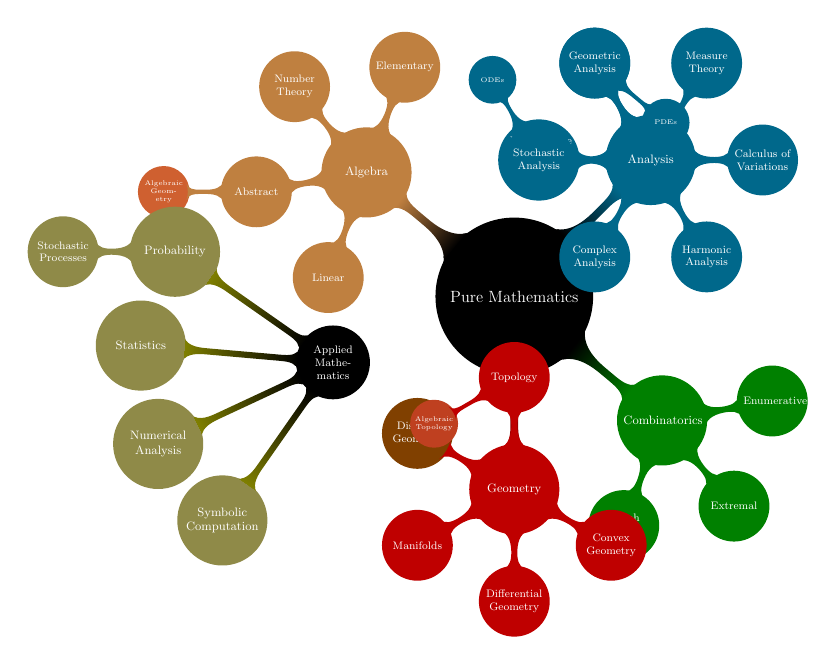
\begin{tikzpicture}[scale=0.49, transform shape]
\path[mindmap,concept color=black,text=white]
node[concept] {Pure Mathematics} [clockwise from=45]
child[concept color=DeepSkyBlue4]{
node[concept] {Analysis} [clockwise from=180]
child {
node[concept] {Multivariate \&amp; Vector Calculus}
[clockwise from=120]
child {node[concept] {ODEs}}}
child { node[concept] {Functional Analysis}}
child { node[concept] {Measure Theory}}
child { node[concept] {Calculus of Variations}}
child { node[concept] {Harmonic Analysis}}
child { node[concept] {Complex Analysis}}
child { node[concept] {Stochastic Analysis}}
child { node[concept] {Geometric Analysis}
[clockwise from=-40]
child {node[concept] {PDEs}}}}
child[concept color=black!50!green, grow=-40]{
node[concept] {Combinatorics} [clockwise from=10]
child {node[concept] {Enumerative}}
child {node[concept] {Extremal}}
child {node[concept] {Graph Theory}}}
child[concept color=black!25!red, grow=-90]{
node[concept] {Geometry} [clockwise from=-30]
child {node[concept] {Convex Geometry}}
child {node[concept] {Differential Geometry}}
child {node[concept] {Manifolds}}
child {node[concept,color=black!50!green!50!red,text=white] {Discrete Geometry}}
child {
node[concept] {Topology} [clockwise from=-150]
child {node [concept,color=black!25!red!50!brown,text=white]
{Algebraic Topology}}}}
child[concept color=brown,grow=140]{
node[concept] {Algebra} [counterclockwise from=70]
child {node[concept] {Elementary}}
child {node[concept] {Number Theory}}
child {node[concept] {Abstract} [clockwise from=180]
child {node[concept,color=red!25!brown,text=white] {Algebraic Geometry}}}
child {node[concept] {Linear}}}
node[extra concept,concept color=black] at (200:5) {Applied Mathematics}
child[grow=145,concept color=black!50!yellow] {
node[concept] {Probability} [clockwise from=180]
child {node[concept] {Stochastic Processes}}}
child[grow=175,concept color=black!50!yellow] {node[concept] {Statistics}}
child[grow=205,concept color=black!50!yellow] {node[concept] {Numerical Analysis}}
child[grow=235,concept color=black!50!yellow] {node[concept] {Symbolic Computation}};
\end{tikzpicture}
\end{document}
\end{lstlisting}

\begin{figure}[htpb]
	\centering
	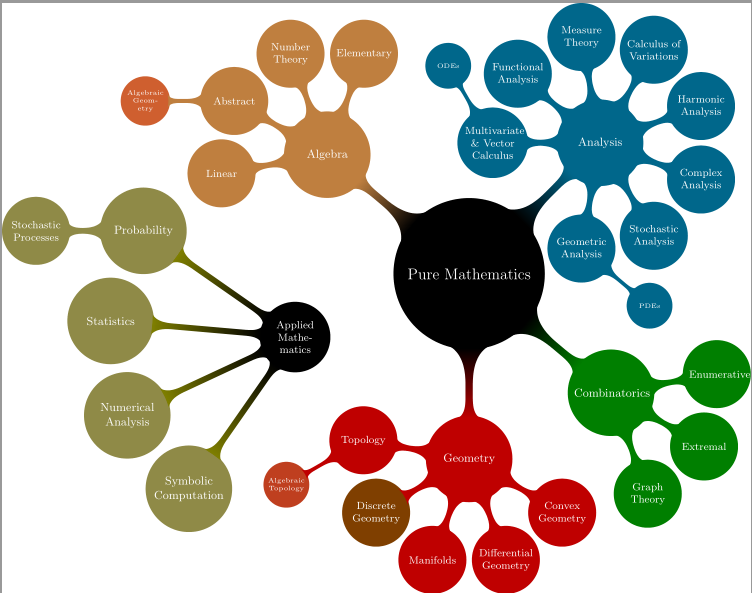
\includegraphics[width=0.4\linewidth]{mindmap.png}
	\caption{使用Tikz制作思维导图示例。}\label{fig:mindmap}
\end{figure}

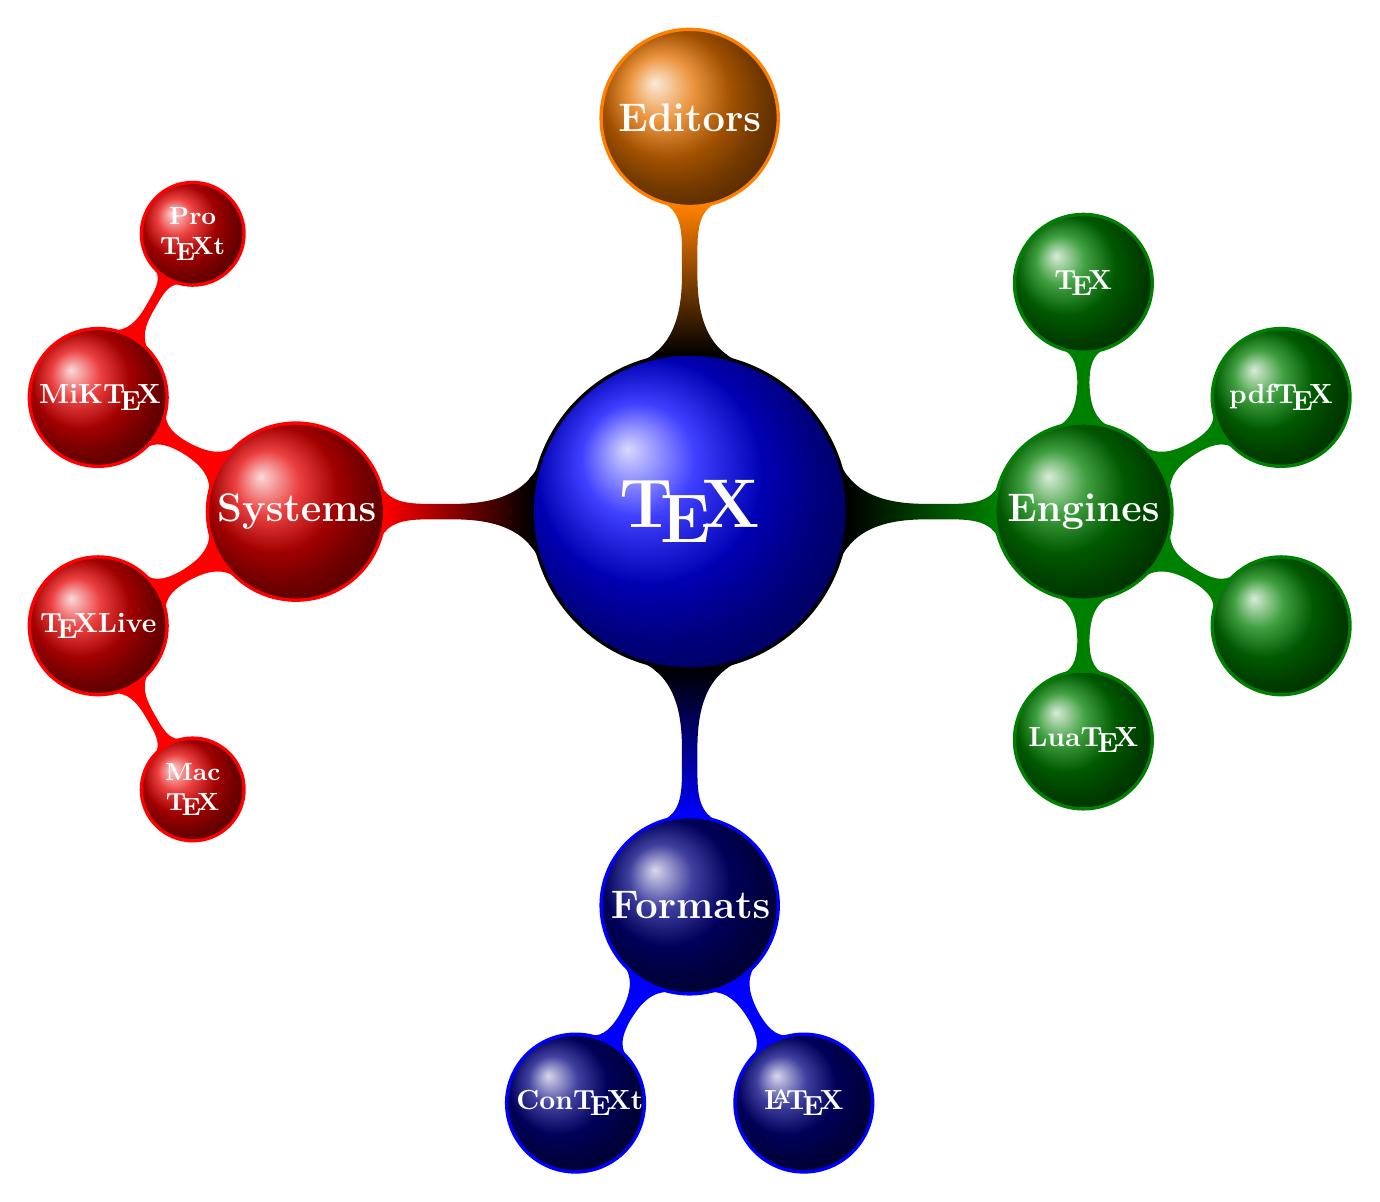
\begin{tikzpicture}
\path [
mindmap,
text = white,
level 1 concept/.append style =
{font=\Large\bfseries, sibling angle=90},
level 2 concept/.append style =
{font=\normalsize\bfseries},
level 3 concept/.append style =
{font=\small\bfseries},
tex/.style     = {concept, ball color=blue,
	font=\Huge\bfseries},
engines/.style = {concept, ball color=green!50!black},
formats/.style = {concept, ball color=blue!50!black},
systems/.style = {concept, ball color=red!90!black},
editors/.style = {concept, ball color=orange!90!black}
]
node [tex] {\TeX} [clockwise from=0]
child[concept color=green!50!black, nodes={engines}] {
	node {Engines} [clockwise from=90]
	child { node {\TeX} }
	child { node {pdf\TeX} }
	child { node {\XeTeX} }
	child { node {Lua\TeX} }}
child [concept color=blue, nodes={formats}] {
	node {Formats} [clockwise from=300]
	child { node {\LaTeX} }
	child { node {Con\TeX t} }}
child [concept color=red, nodes={systems}] {
	node {Systems} [clockwise from=210]
	child { node {\TeX Live} [clockwise from=300]
		child { node {Mac \TeX} }}
	child { node {MiK\TeX} [clockwise from=60]
		child { node {Pro \TeX t} }}}
child [concept color=orange, nodes={editors}] {
	node {Editors} };
\end{tikzpicture}

\begin{tikzpicture}[mindmap,scale=0.9]
\begin{scope}[
every node/.style={concept,circular drop shadow,execute at begin node=\hskip0pt},
root concept/.append style={
	concept color=black,fill=white,line width=1ex,text=black,font=\large\scshape},
text=white,yi/.style={concept color=red,faded/.style={concept color=red!50}},
er/.style={concept color=blue,faded/.style={concept color=blue!50}},
san/.style={concept color=orange,faded/.style={concept color=orange!50}},
si/.style={concept color=green!50!black,faded/.style={concept color=green!50!black!50}},
wu/.style={concept color=db,faded/.style={concept color=db!50}},
grow cyclic,
level 1/.append style={level distance=5.5cm,sibling angle=90,font=\scshape},
level 2/.append style={level distance=3.2cm,sibling angle=38,font=\scriptsize}
]
\node[root concept]at (current page.center){\Large 数专考纲\\mindmap}
% [clockwise from=90]
child[yi]{node{\large 数学分析}%[clockwise from=145]
	child{node{极限与连续}}
	child{node{一元函数微积分\\及其应用}}
	child{node{多元函数微分学}}
	child{node{级数理论\\与广义积分}}
}
child[er]{node{\large 英语一}
	child{node{无}}
	child{node{无}}
	child{node{无}}
	child{node{无}}
}
child[san]{node{\large 政治}%[clockwise from=0]
	child{node{无}}
	child{node{无}}
	child{node{无}}
	child{node{无}}
}
child[si]{node{\large 高等代数}%[clockwise from=-60]
	child{node{高等代数}}
	child{node{行列式理论}}
	child{node{线性方程组理论}}
	child{node{矩阵理论}}
	child{node{二次型理论}}
	child{node{线性空间理论}}
	child{node{线性变换理论}}
	child{node{欧式空间理论}}
};
\end{scope}
\end{tikzpicture}